\documentclass[twoside,a5paper,10pt,openright]{memoir}
% \setstocksize{230mm}{160mm}
\setlrmarginsandblock{3cm}{2cm}{*}
\setulmarginsandblock{2cm}{2cm}{*}
\checkandfixthelayout

\usepackage[utf8]{inputenc}
\usepackage[english]{babel}
\usepackage[style=authoryear]{biblatex}
\addbibresource{references.bib}

\usepackage{amsmath}
\usepackage{hyperref}
\usepackage{fontspec}
\usepackage{unicode-math}
\usepackage{graphicx}
\usepackage[super]{nth}
\usepackage{booktabs}
\usepackage{csquotes}
\usepackage{multirow}
\usepackage{cleveref}
%\usepackage[Glenn]{fncychap}
\usepackage{tikz}
\usepackage{titling}
\usepackage{tcolorbox}
\usepackage{xhfill}

\usepackage{qrcode}
\newcommand{\linkwithqr}[1]{%
  \begin{minipage}{0.8\textwidth}
    \url{#1}
  \end{minipage}
  \hfill
  \begin{minipage}{0.15\textwidth}
    \qrcode[height=\textwidth]{#1}
  \end{minipage}
}

\nonfrenchspacing

\begin{document}

\setmathfont{STIXTwoMath}[
  Extension={.otf},
  Path={./fonts/},
  Scale=1]

\setmainfont{STIXTwoText}[
  Extension={.otf},
  Path={./fonts/},
  UprightFont={*-Regular},
  BoldFont={*-Bold},
  ItalicFont={*-Italic},
  BoldItalicFont={*-BoldItalic}]

% Change figure and table captions font size.
\captionnamefont{\small}
\captiontitlefont{\small}

\tcbset {
  base/.style={
    arc=0mm,
    bottomtitle=0.5mm,
    boxrule=0mm,
    colbacktitle=black!20!white,
    coltitle=black,
    fonttitle=\bfseries,
    left=2.5mm,
    leftrule=1mm,
    right=3.5mm,
    title={#1},
    toptitle=0.75mm,
  }
}

\newtcolorbox{mainbox}[1]{
  colframe=black!20!white,
  base={#1}
}

\newcommand\boxsubtitle[1]{%
  \vspace{0.5em}
  \noindent\xrfill[0.5ex]{1pt}[black!20]\phantom{x}\textbf{#1}\phantom{x}\xrfill[0.5ex]{1pt}[black!20]%
  \vspace{0.5em}
}

\renewcommand{\vec}[1]{\mathbf{#1}}

\title{Data science: foundations and practices}
\author{Filipe A. N. Verri}

\hypersetup{%
  pdftitle={\thetitle},
  pdfsubject={Data science},
  pdfauthor={\theauthor},
  pdfkeywords={data science, statistics, machine learning, databases}}

\maketitle
\thispagestyle{empty}
\clearpage

\newpage
\mbox{}
\vfill

{
\footnotesize
Scripture quotations are from The ESV® Bible (The Holy Bible, English Standard Version®),
copyright © 2001 by Crossway, a publishing ministry of Good News Publishers. Used by
permission. All rights reserved.
}

\vspace{0.5cm}
{
\footnotesize
\thetitle{} © \the\year{} by \theauthor{} is licensed under
Attribution-NonCommercial-NoDerivatives 4.0 International. To view a copy of this license,
visit
\href{http://creativecommons.org/licenses/by-nc-nd/4.0/}{creativecommons.org/licenses/by-nc-nd/4.0}.
}

\thispagestyle{empty}
\newpage

\tableofcontents
\thispagestyle{empty}

\chapter{About this book}

\begin{parwithqr}{https://github.com/verri/dsp-book}
  I intend to make this book forever free and open-source. You can find (and contribute
  to) the source code at \href{\aurl}{github.com/verri/dsp-book}.
\end{parwithqr}

\vfill

\begin{parwithqr}{https://www.buymeacoffee.com/verri}
  If you like this book, consider \emph{buying me a coffee} at
  \href{\aurl}{buymeacoffee.com/verri}.   All donations are used to improve this book,
  including editing and proofreading.
\end{parwithqr}

\vfill

\begin{parwithqr}{https://github.com/verri/dsp-book/issues}
  If you find any typos, grammar errors, incomplete material or have any suggestions,
  please open an issue at \href{\aurl}{github.com/verri/dsp-book/issues}.
\end{parwithqr}

\vfill

\begin{parwithqr}{https://comp.ita.br/\~verri/ds-book-print}
  Students can found a printable version (A4 paper, double-sided, short-edge spiral
  binding) of this book at \href{\aurl}{comp.ita.br/\textasciitilde{}verri/ds-book-print}.
\end{parwithqr}

\newpage
This book comprises the lectures notes of the course PO-235 Data Science Project.
I hope someday it becomes an actual book. For now, beware many typos, grammar errors, ugly
typesetting, disconnected material, etc.

Also, it is important to highlight that:
\begin{itemize}
  \item This is not a Machine Learning book, and I do not intend to explain how specific
    ML algorithms work.
  \item This contains some kind of introductory material on data science.  Although I
    introduce the fundamental concepts, I expect you have strong mathematical and
    statistics background.
  \item An artificial constraint I have imposed in the material (for the sake of the
    course) is that I only consider \emph{predictive methods}, more specifically
    inductive ones. I not address topics such as clustering, association-rules
    mining, transductive learning, anomaly detection, time series forecasting, reinforced
    learning, etc.
\end{itemize}

I have decided to work on this material because the books I like on data science are
either
\begin{itemize}
  \item too broad and too shallow, in the sense they hide many mathematical foundations
    and focus on just explaining what data science is and where it is applied;
  \item too tool-centric, in the sense that they focus only on a specific toolbox or
    programming language; or
  \item too machine-learning-y, exposing many machine learning algorithms and missing the
    foundations of learning.
\end{itemize}

So\dots, I expect my approach on the subject provide:
\begin{itemize}
  \item awareness of all steps in a data science project;
  \item deeper focus (than most books) on data transformation, describing the semantics of dataset
    operators instead of restraining ourselves with a specific tool;
  \item deeper focus (than most books) on why machine learning works, increasing awareness of its pitfalls and
    limitations;
  \item deeper focus (than most books) on correct evaluation and validation
    (pre-deployment) of machine learning models.
\end{itemize}

This book covers the following material:
\begin{itemize}
  \item Brief history of data science.
  \item Background topics.
  \item Fundamental data concepts.
  \item Stages in a data science project.
  \item Data Infrastructure.
  \item Data integration from multiple sources.
  \item Data engineering and shaping.
  \item Inductive learning and principles of statistical learning theory.
  \item Application of Machine Learning models in real-world problems.
  \item Experimental planning for data science.
  \item Model evaluation and Bayesian analysis.
  \item Documentation and deployment.
  \item Ethical and legal issues in data science.
  \item Privacy-preserving computational approaches.
\end{itemize}

\chapter*{Course plan}

For administrative reasons, I present the course plan for PO-235 and CMC-16.

\newpage
\newgeometry{margin=1cm}
\thispagestyle{empty}
\section*{PO-235 Data science project}

\emph{Course plan (\the\year{})}

Prof. Filipe A. N. Verri

\paragraph{Number of students:} Approx. 20 (hopefully close to 10)

\paragraph{Course load:} 3--0--0--4

\paragraph{Requirements:} Advanced programming skills, strong statistics background, and
beginner level machine learning skills.

\paragraph{Course program:}
Brief history of data science.  Fundamental data concepts. Stages in a Data Science
project.  Data Infrastructure. Data integration from multiple sources. Data engineering
and shaping.  Inductive learning and principles of statistical learning theory.
Application of machine learning models in real-world problems.  Experimental planning for
data science. Model evaluation and Bayesian analysis.  Documentation and deployment.
Ethical and legal issues in data science.  Privacy-preserving computational approaches.

\paragraph{Goals:}
Providing the theoretical background and the practical concepts to develop an end-to-end
data science project for an inductive task.

\paragraph{Teaching methodology:}
Expository classes in common classroom, using whiteboard, slide presentations, coding
examples, books and scientific papers. Supplementary didactic materials will be available
in Google Classroom. The development of the case study will happen during home study
hours, including programming and scientific paper writing.

\paragraph{Grading:} Two individual written tests in the \nth{1} and another in the \nth{2} quarter.
Scientific paper and oral presentation about the case study for the final exam.

\paragraph{Bibliography:}
\begin{itemize}
  \item Nina Zumel and John Mount. Practical Data Science with R. Manning, 2nd Edition, 2019.
  \item Hadley Wickham and Garret Grolemund, R for Data Science: Import, Tidy, Transform, Visualize, and Model Data. O’Reilly Media, 2017.
  \item John D. Kelleher and Brendan Tierney. Data science, MIT Press, 2018.
\end{itemize}

\paragraph{Must read:}
\begin{itemize}
  \item In-progress textbook at \url{https://comp.ita.br/~verri/dsp-book}.
  \item \fullcite{Vapnik1999}.
  \item \fullcite{Benavoli2017}.
\end{itemize}
\thispagestyle{empty}

\paragraph{Calendar:} The expected schedule is presented below.

\begin{center}
  \begin{tabular}{ll}
    \toprule
    \multicolumn{2}{c}{\bf \nth{1} Quarter} \\
    \midrule
    Week & Topics \\
    \midrule
    \multirow{2}{*}{1} & Brief history of data science (\cref{chap:history}) \\
      & Peliminaries (\cref{chap:preliminaries})\\
    \midrule
    2 & \bf Written test \\
    \midrule
    \multirow{2}{*}{3} & Fundamental data concepts (\cref{chap:data}) \\
      & Stages in a data science project \\
    \midrule
    4 & \multirow{2}{*}{Inductive learning and statistical learning theory} \\
    5 &  \\
    \midrule
    6 & Data infrastructure and data integration from multiple sources \\
    \midrule
    7 & Data engineering and shaping \\
    \midrule
    8 & \bf Written test \\
    \bottomrule
  \end{tabular}
\end{center}

\begin{center}
  \begin{tabular}{ll}
    \toprule
    \multicolumn{2}{c}{\bf \nth{2} Quarter} \\
    \midrule
    Week & Topics \\
    \midrule
    1 & \multirow{2}{*}{Application of machine learning models in real-world problems} \\
    2 &  \\
    \midrule
    3 & \multirow{2}{*}{Experimental planning for data science} \\
    4 & \\
    \midrule
    5 & \multirow{2}{*}{Model evaluation and Bayesian analysis} \\
    6 & \\
    \midrule
    7 & \bf Written test \\
    \midrule
    \multirow{3}{*}{8} & Documentation and deployment \\
      & Ethical and legal issues in data science \\
      & Privacy-preserving computational approaches \\
    \bottomrule
  \end{tabular}
\end{center}

Case studies will be presented during exam weeks.

\newpage
\newgeometry{margin=1cm}
\thispagestyle{empty}
\section*{CMC-16 Data science practices}

\emph{Course plan (\the\year{})}

\nth{1} Semester of \the\year{}

Prof. Filipe A. N. Verri

\paragraph{Number of students:} Approx. 20

\paragraph{Course load:} 2--0--1--5

\paragraph{Requirements:} CMC-13 or CMC-15

\paragraph{Course program:}
Brief history of Data Science. Stages in a Data Science project. Tidy Data. Data
integration from multiple sources. Data engineering and shaping. Inductive learning and
statistical learning theory. Experimental planning for Data Science. Model evaluation and
Bayesian Analysis. Documentation and deployment. Privacy-preserving computational
approaches.

\paragraph{Goals:}
Further studying the practical aspects of Data Science (in relation to CMC-13) and providing
the mathematical foundations to ensure the correct usage of Data Science techniques.

The specific goals are:
\begin{itemize}
  \item Understanding the steps and people involved in Data Science projects;
  \item Developing an end-to-end case study, including data collection, data transformation,
    inductive learning, validation, documentation, and deployment; and
  \item Critically evaluate the results and implications of the case study.
\end{itemize}

\paragraph{Teaching methodology:}
Expository classes in common classroom, using whiteboard, slide presentations, coding
examples, books and scientific papers. Supplementary didactic materials will be available
in Google Classroom. The development of the case study will happen during laboratory
classes and home study hours, including programming and writing essays.

\paragraph{Grading:} One individual written test in the \nth{1} and another in the \nth{2} quarter.
Essay and oral presentation about the case study (in groups) for the final exam.

\paragraph{Bibliography:}
\begin{itemize}
  \item Nina Zumel and John Mount. Practical Data Science with R. Manning, 2nd Edition, 2019.
  \item Hadley Wickham and Garret Grolemund, R for Data Science: Import, Tidy, Transform, Visualize, and Model Data. O’Reilly Media, 2017.
  \item John D. Kelleher and Brendan Tierney. Data Science, MIT Press, 2018.
\end{itemize}

\thispagestyle{empty}
\paragraph{Recommended reading:}
\begin{itemize}
  \item In-progress textbook at \url{https://comp.ita.br/~verri/dsp-book}.
  \item \fullcite{Vapnik1999}.
  \item \fullcite{Benavoli2017}.
\end{itemize}

\paragraph{Calendar:} The expected schedule is presented below.

\begin{center}
  \begin{tabular}{ll}
    \toprule
    \multicolumn{2}{c}{\bf \nth{1} Quarter} \\
    \midrule
    Week & Topics \\
    \midrule
    1 & Brief history of Data Science and CMC-13 review \\
    2 & Stages in a Data Science project \\
    3 & Tidy Data and data integration from multiple sources \\
    4 & Data engineering and shaping \\
    5 & \multirow{2}{*}{Inductive learning and statistical learning theory} \\
    6 &  \\
    7 & Case study discussion and definitions \\
    8 & \bf Written test \\
    \bottomrule
  \end{tabular}
\end{center}

\begin{center}
  \begin{tabular}{ll}
    \toprule
    \multicolumn{2}{c}{\bf \nth{2} Quarter} \\
    \midrule
    Week & Topics \\
    \midrule
    1 & Experimental planning for Data Science \\
    2 & Model evaluation \\
    3 & Bayesian Analysis \\
    4 & Documentation and deployment \\
    5 & Privacy-preserving computational approaches \\
    6 & \bf Written test \\
    7 & \multirow{2}{*}{\bf Presentations and discussions} \\
    8 & \\
    \bottomrule
  \end{tabular}
\end{center}

\restoregeometry
\thispagestyle{empty}

\chapter{Brief history of data science}
\label{chap:history}

\chapterprecishere{``Begin at the beginning,'' the King said gravely, ``and
go on till you come to the end: then stop.''\par\raggedleft--- \textup{Lewis
Carroll}, Alice in Wonderland}

There are many points-of-view about the beginning of data science.  For the sake of
contextualization, I separate the topic in two approaches: the history of the term itself
and a broad timeline of data-driven sciences highlighting the important figures in each
age.

\begin{mainbox}{Chapter remarks}
  \boxsubtitle{Context}

  \begin{itemize}
    \item The term ``data science'' is recent and has been used to label rather different fields.
    \item The history of data-driven sciences is long and rich.
  \end{itemize}

  \boxsubtitle{Objectives}

  \begin{itemize}
    \item Understand the history of the term ``data science.''
    \item Understand the history of data-driven sciences.
  \end{itemize}

  \boxsubtitle{Takeways}

  \begin{itemize}
    \item There is no consensus on the definition of data science.
    \item There is enough evidence to support data science as a new science.
  \end{itemize}
\end{mainbox}

\section{The term ``data science''}

The term data science is recent and has been used to label rather different fields of
study.  In the following, I emphasize the history of a few notable usage of the term.

\def\naurds{(0,0) circle (20mm)}
\def\naurcs{(0:5mm) circle (15mm)}
\def\naurde{(0:40mm) circle (15mm)}

\colorlet{circle edge}{black!50}
\colorlet{circle area}{black!20}

\tikzset{filled/.style={fill=circle area, draw=circle edge, thick},
    outline/.style={draw=circle edge, thick}}

\begin{figurebox}[label=fig:naur]{Naur's view of data science.}
  \centering
  \begin{tikzpicture}
    \begin{scope}
      \clip \naurds;
      \fill[filled] \naurcs;
    \end{scope}
    \draw[outline] \naurds node(ds) {};
    \draw[outline] \naurcs node {computer science};
    \draw[outline] \naurde node {domain expertise};
    \node[anchor=north,above] at (0,2) {data science};
  \end{tikzpicture}
  \tcblower
    For him, data science studies the techniques to deal
    with data, but he delegates the meaning of data to other fields.
\end{figurebox}

\paragraph{Peter Naur (1928 -- 2016)}

The term ``data science'' itself was coined in the 1960s by Peter Naur (/naʊə/). Naur was
a Danish computer scientist and mathematician who made significant contributions to the
field of computer science, including his work on the development of programming
languages\footnote{He is best remembered as a contributor, with John Backus, to the
Backus–Naur form (BNF) notation used in describing the syntax for most programming
languages.}.
His ideas and concepts laid the groundwork for the way we think about programming and data
processing today.

\begin{mainbox}{Peter Naur}
  \begin{itemize}
    \item Danish computer scientist and mathematician.
    \item Coined the term ``data science'' in the 1960s.
    \item Proposed the term ``datalogy'' as an alternative to computer science.
  \end{itemize}
\end{mainbox}

Naur disliked the term computer science and suggested it be called datalogy or data
science.  In the 1960s, the subject was practised in Denmark under Peter
Naur's term datalogy, which means the science of data and data processes.

He coined this term to emphasize the importance of data as a fundamental component of
computer science and to encourage a broader perspective on the field that included
data-related aspects. At that time, the field was primarily centered on programming
techniques, but Naur's concept broadened the scope to recognize the intrinsic role of data
in computation.

In his book\footnote{Peter Naur: Concise Survey of Computer Methods, 397 p.
Studentlitteratur, Lund, Sweden, ISBN 91-44-07881-1, 1974.
\url{http://www.naur.com/Conc.Surv.html}}, ``Concise Survey of Computer Methods'', he
parts from the concept that \emph{data} is ``a representation of facts or ideas in a
formalised manner capable of being communicated or manipulated by some
process.''\footnote{I. H. Gould (ed.): ‘IFIP guide to concepts and terms in data
processing’, North-Holland Publ. Co., Amsterdam, 1971.} Note however that his view of the
science only ``deals with data [\dots] while the relation of data to what they represent
is delegated to other fields and sciences.''

\def\clevelandds{(0,0) circle (20mm)}
\def\clevelandst{(0:-5mm) circle (15mm)}
\def\clevelandde {(2,1) circle (15mm)}
\def\clevelandcs {(2,-1) circle (15mm)}

\begin{figurebox}[label=fig:cleveland]{Cleveland's view of data science.}
  \centering
  \begin{tikzpicture}
    \begin{scope}
      \clip \clevelandds;
      \fill[filled] \clevelandst;
      \fill[filled] \clevelandde;
      \fill[filled] \clevelandcs;
    \end{scope}
    \draw[outline] \clevelandds node(ds) {};
    \draw[outline] \clevelandst node {statistics};
    \draw[outline] \clevelandde node {domain expertise};
    \draw[outline] \clevelandcs node {computer science};
    \node[anchor=north,above] at (0,2) {data science};
  \end{tikzpicture}
  \tcblower
    For him, data science is the ``modern'' statistics,
    where it is enlarged by computer science and domain expertise.
  \label{fig:cleveland}
\end{figurebox}

\paragraph{William Cleveland (born 1943)}

In 2001, a prominent statistician used the term ``data science" in his work to describe a
new discipline that comes from his ``plan to enlarge the major areas of technical work of
the field of statistics\footnote{W. S. Cleveland. Data Science: An Action Plan for
Expanding the Technical Areas of the Field of Statistics. ISI Review, 69:21–26, 2001.}.''
In 2014, that work was republished\footnote{W. S. Cleveland.
Data Science: An Action Plan for the Field of Statistics. Statistical Analysis and Data
Mining, 7:414–417, 2014. reprinting of 2001 article in ISI Review, Vol 69.}.
He advocates the expansion of statistics beyond theory into technical areas, significantly
changing statistics.  Thus, it warranted a new name.

\begin{mainbox}{William Cleveland}
  \begin{itemize}
    \item American statistician.
    \item Proposed the discipline ``data science'' in 2001.
    \item Proposed the term ``data science'' as the new name for expansion of statistics.
  \end{itemize}
\end{mainbox}

As a result, William Swain Cleveland II is credited to define data science as it is most
used today. He is a highly influential figure in the fields of statistics, machine
learning, data visualization, data analysis for multidisciplinary studies, and high
performance computing for deep data analysis.

\paragraph{Buzzword or a new science?}

Be aware that literature has no consensus on the definition of data science, and it is still considered
by some to be a buzzword\footnote{Press, Gil. "Data Science: What's The Half-Life of a
Buzzword?". Forbes. Available at
\url{https://www.forbes.com/sites/gilpress/2013/08/19/data-science-whats-the-half-life-of-a-buzzword/}}.

Most of the usages of the term in literature and in the media are either a rough
reference to a set of data-driven techniques or a marketing strategy.  Naur
(\cref{fig:naur}) and Cleveland (\cref{fig:cleveland}) are among the few that try to
carefully define the term.  However, both of them do not see data science as an
independent field of study, but an enlarged scope of an existing science.  I disagree;
the social and economical demand for data-driven solutions led to an evolution in our
understanding of the challenges we are facing.  As a result, we see many ``data
scientist'' being hired and many ``data science degrees'' programs emerging.

In \cref{chap:data}, I dare to provide a (yet another) definition for the term.  I
argue that its object of study can be precisely established to support it as a new
science.

\begin{mainbox}{A new science}
  \begin{itemize}
    \item Both Naur and Cleveland do not see data science as an independent field of study.
    \item I argue that data science is not a buzzword.
    \item Our social and economical reality demands a new science.
  \end{itemize}
\end{mainbox}

\section{Timeline and historical markers}

\textcite{Kelleher2018} provides an interesting time line of data-driven methods and
influential figures in the field.  I reproduce it here with some changes, including
some omissions and additions.

I first address data handling --- which I include data sources, collection, organization,
storage, and manipulation ---, and then data analysis and knowledge extraction.

\subsection{Timeline of data handling}

The importance of collecting and organizing data goes without saying.  Data fuels analysis and
decision making.  In the following, I present some of the most important milestones in the history
of data handling.

\begin{figurebox}[label=fig:data-handling-history]{Timeline of the ages of data handling.}
  \centering
  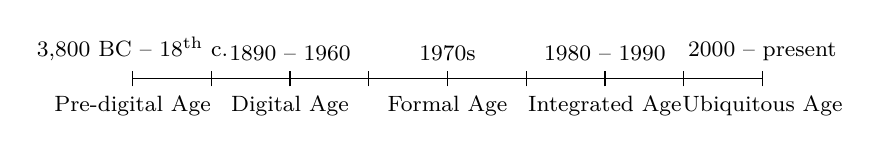
\begin{tikzpicture}
    \draw (0,0) -- (8,0);
    \foreach \x in {0,1,...,8} {
      \draw (\x,-0.1) -- (\x,0.1);
    }
    \foreach \x/\y/\z in {%
        0/Pre-digital Age/{3,800 BC -- \nth{18} c.},
        2/Digital Age/{1890 -- 1960},
        4/Formal Age/{1970s},
        6/Integrated Age/{1980 -- 1990},
        8/Ubiquitous Age/{2000 -- present}} {
      \node[anchor=north] at (\x,-0.1) {\footnotesize\y};
      \node[anchor=south] at (\x,0.1) {\footnotesize\z};
    }
  \end{tikzpicture}
\end{figurebox}

\Cref{fig:data-handling-history} illutrates the timeline.

\subsubsection{Pre-digital age}

We can consider the earliest records of data collection to be the notches on sticks and
bones to keep tracking of passing of time.  The Lebombo bone, a baboon fibula with
notches, is probably the earliest known mathematical object.  It was found in the Lebombo
Mountains located between South Africa and Eswatini.
They estimate it is more
than 40,000 years old. It is conjectured to be a tally stick, but its exact purpose is
unknown. Its 29 notches suggests that may have been used as a lunar phase counter.
However, since it is broken at one end, the 29 notches may or may not be the total
number\footcite{Beaumont2013}.

Another important milestone in the history of data collection is the record of
demographic data.  One of first known census was conducted in 3,800 BC in the Babylonian
Empire.  It was ordered to assess the population and resources of
his empire.  Records were stored on  clay  tiles\footcite{Grajalez2013}.

Since the early forms of writing, humanity abilities to record events and information
increased significantly.  The first known written records date back to around 3,500 BC, the
Sumerian archaic (pre-cuneiform) writing.  This writing system was used to represent
commodities using clay tokens and to record transactions\footcite{Ifrah1998}.

``Data storage'' was also a challenge.  Some important devices that increased our capacity
to register textual information are the Sumerian clay tablets (3,500 BC), the Egyptian
papyrus (3,000 BC), the Greek alphabet (800 BC), the Roman wax tablets (100 BC), the codex
(100 AD), the Chinese paper (200 AD), the printing press (1440), the typewriter (1868).

% Talvez citar na parte de análise de dados
% Other mechanisms were also developed to store information in a more structured way.  Some
% important devices are
% the abacus (2,700 BC), the Antikythera mechanism (150 -- 100 BC), the
% Chinese South Pointing Chariot (260 AD), the Pascaline (1642), the Jacquard loom (1801),
% the Babbage Difference Engine (1822), the Babbage Analytical Engine (1837).

Besides those improvements in unstructured data storage, at least in the Western and
Middle Eastern world, there are no significant advances in structured data collection
until the \nth{19} century.  (A Eastern timeline research is pending.)

I consider a major influential figure in the history of data
collection to be Florence Nightingale (1820 -- 1910).  She was a passionate statistician
and probably the first person to use statistics to influence public and official
opinion.  The meticulous records she kept during the Crimean War
(1853 -- 1856) were the evidence that saved lives.  She was also the first to use
statistical graphics to present data in a way that was easy to understand.  She is
credited with developing a form of the pie chart now known as the polar area
diagram.  She also reformed healthcare in the United Kingdom and
is considered the founder of modern nursing\footcite{Grajalez2013}.

\begin{mainbox}{Florence Nightingale}
  \begin{itemize}
    \item Passionate statistician.
    \item First person to use statistics to influence public and official opinion.
    \item Organized data from garden fruits and vegetables into numerical tables at the age of 9.
    \item At 20 she was receiving two-hour lessons from a Cambridge-trained mathematician.
    \item She found the sight of a long column of figures ``perfectly reviving.''
    \item She went out to the Crimean War, to Scutari in Turkey, in 1854.
    \item She found that not even the numbers of soldiers entering the hospitals, or leaving them – alive or dead – was known.
    \item From the first she kept meticulous records.
    \item The data she collected was the evidence that saved lives.
    \item She was the first to use statistical graphics to present data in a way that was easy to understand.
    \item She is credited with developing a form of the pie chart now known as the polar area diagram.
    \item She reformed healthcare in the United Kingdom and is considered the founder of modern nursing.
  \end{itemize}
\end{mainbox}

\begin{mainbox}{Pre-digital age}
  \begin{itemize}
    \item Babylonian census (3,800 BC)
    \item Sumerian archaic (pre-cuneiform) writing (3,500 BC)
    \item Egyptian papyrus (3,000 BC)
    \item Phoenician alphabet (1,000 BC)
    \item Greek alphabet (800 BC)
    \item Roman wax tablets (100 BC)
    \item Codex (100 AD)
    \item Chinese paper (200 AD)
    \item Printing press (1440)
    \item Typewriter (1868)
    \item Florence Nightingale (1820 -- 1910)
  \end{itemize}
\end{mainbox}

\subsubsection{Digital age}

In the modern period, several devices were developed to store digital\footnote{Digital
means the representation of information in (finite) discrete form.  The term comes from the Latin
digitus, meaning finger, because it is the natural way to count using fingers.}
information.  One particular device that is important for data collection is the punched
card.  It is a piece of stiff paper that contains digital information represented by the
presence or absence of holes in predefined positions.  The information can be read by a
mechanical or electrical device called a card reader.  The earliest famous usage of
punched cards was by Basile Bouchon (1725) to control looms.  Most of the advances until
the 1880s were about the automation of machines (data processing) using hand-punched cards, and not
particularly specialized for data collection.

However, the 1890 census in the United States was the first to use machine-readable
punched cards to tabulate data. Processing 1880 census data took eight years, so the
Census Bureau contracted Herman Hollerith (1860 -- 1929) to design and build a tabulating
machine.  He founded the Tabulating Machine Company in 1896, which later merged with other
companies to become International Business Machines Corporation (IBM) in 1924. Later
models of the tabulating machine were widely used for business applications such as
accounting and inventory control. Punched card technology remained a prevalent method of
data processing for several decades until more advanced electronic computers were
developed in the mid-\nth{20} century.

The invention of the digital computer is responsible for a revolution in data handling.
The amount of information we can capture and store increased exponentially.  ENIAC (1945) was
the first electronic general-purpose computer.  It was Turing-complete, digital, and
capable of being reprogrammed to solve a full range of computing problems.
It had 20 words of internal memory, each capable of storing a 10-digit decimal integer number.
Programs and data were entered by setting switches and inserting punched cards.

For the 1950 census, the United States Census Bureau used the
UNIVAC I (Universal Automatic Computer I), the first commercially produced computer in the
United States\footnote{Read more in \url{https://www.census.gov/history/www/innovations/}.}.

It goes without saying that digital computers have become much more powerful and
sophisticated since then.  The data collection process has been easily automated and
scaled to a level that was unimaginable before.  However, ``where'' storing data is
not the only challenge.  ``How'' to store data is also a challenge.  The next period of
history addresses this issue.

\begin{mainbox}{Digital age}
  \begin{itemize}
    \item Punched card (1725)
    \item 1890 census and Hollerith's tabulating machine (1890)
    \item ENIAC (1945)
    \item UNIVAC I used by the United Census Bureau (1950)
  \end{itemize}
\end{mainbox}

\subsubsection{Formal age}

In 1970, Edgar Frank Codd (1923 -- 2003) published a paper entitled ``A Relational Model
of Data for Large Shared Data Banks''\footcite{Codd1970}.  In this paper, he introduced
the concept of a relational model for database management {\color{red}
provide more details}.

His work was a breakthrough in the field of data management.  The standardization of
relational databases led to the development of Structured Query Language (SQL) in 1974.
SQL is a domain-specific language used in programming and designed for managing data held
in a relational database management system (RDBMS).

As a result, a new challenge rapidly emerged: how to aggregate data from different
sources. Once data is stored in a relational database, it is easy to query and manipulate
it. However, data is usually stored in different databases, and it is not always possible
to combine them.

\begin{mainbox}{Edgar Frank Codd}
  \begin{itemize}
    \item British computer scientist.
    \item Introduced the concept of a relational model for database management.
    \item Standardized relational databases.
    \item Led the development of Structured Query Language (SQL).
  \end{itemize}
\end{mainbox}

\subsubsection{Integrated age}

The solution to this problem was the development of the Extract, Transform, Load (ETL)
process.  ETL is a process in data warehousing responsible for extracting data from
several sources, transforming it into a format that can be analyzed, and loading it into a
data warehouse.

The concept of data warehousing dates back to the late 1980s when IBM researchers Barry
Devlin and Paul Murphy developed the "business data warehouse"

\textcolor{red}{
Two major figures in the history of ETL are Ralph Kimball and Bill Inmon.  Although they
differ in their approaches, they both agree that data warehousing is the foundation for
business intelligence (BI) and analytics, and that data warehouses should be designed to
be easy to understand and fast to query for business users.
}

\textcolor{red}{
A famous debate between Kimball and Inmon is the top-down versus bottom-up approach to
data warehousing.  Inmon's approach is top-down, where the data warehouse is designed
first and then the data marts are created from the data warehouse.  Kimball's approach is
bottom-up, where the data marts are created first and then the data warehouse is created
from the data marts.
}

\begin{mainbox}{Ralph Kimball}
  \begin{itemize}
    \item American computer scientist.
    \item Developed the bottom-up approach to data warehousing.
  \end{itemize}
\end{mainbox}

\begin{mainbox}{Bill Inmon}
  \begin{itemize}
    \item American computer scientist.
    \item Developed the top-down approach to data warehousing.
  \end{itemize}
\end{mainbox}

\textcolor{red}{
One of the earliest and most famous case studies of the implementation of a data warehouse
is that of Walmart. In the early 1990s, Walmart faced the challenge of managing and
analyzing vast amounts of data from its stores across the United States. The company
needed a solution that would enable comprehensive reporting and analysis to support
decision-making processes.
}

\subsubsection{Ubiquitous age}

The last and current period of history is the ubiquitous age.  It is characterized by the
proliferation of data sources.

The ubiquity of data generation and the evolution of data-centric technologies have been
made possible by a multitude of figures across various domains.

\begin{itemize}
  \item Tim Berners-Lee, credited with inventing the World Wide Web, laid the foundation
    for the massive data flow on the internet.
  \item Vinton Cerf and Robert Kahn, often referred to as the ``Fathers of the Internet,''
    developed the TCP/IP protocols, which are fundamental to internet communication.
  \item Steve Jobs and Steve Wozniak (Apple Inc.) and Bill Gates (Microsoft Corporation),
    the introduction of personal computers, leading to the democratization of data
    generation.
  \item Mark Zuckerberg, the co-founder of Facebook, played a crucial role in the rise of
    social media and the generation of vast amounts of user-generated content.
  \item Larry Page and Sergey Brin, the founders of Google, transformed how we access and
    search for information.
  \item Elon Musk and Tesla, the rise of the Internet of Things (IoT) and connected
    devices.
\end{itemize}

In terms of data handling, this change in the data landscape has brought about the
development of new technologies and techniques for data storage and processing.  Especially
the development of NoSQL databases and distributed computing frameworks.

NoSQL databases are non-relational databases that can store and process large volumes of
unstructured, semi-structured, and structured data.  They are highly scalable and
flexible, making them ideal for big data applications.

\begin{mainbox}{The V's of big data}
  \begin{itemize}
    \item Volume: The amount of data generated is massive.
    \item Velocity: The speed at which data is generated is high.
    \item Variety: The types of data generated are diverse.
    \item Veracity: The quality of data generated is questionable.
    \item Value: The value of data generated is high.
  \end{itemize}
\end{mainbox}

Once massive amounts of unstructured data became available, the need for new data
processing techniques arose.  The development of distributed computing frameworks such as
Apache Hadoop and Apache Spark enabled the processing of massive amounts of data in a
distributed manner.

Doug Cutting and Mike Cafarella, the developers of Apache Hadoop, revolutionized big data
proposed the Hadoop Distributed File System (HDFS) and MapReduce, which are the
cornerstones of the Hadoop framework, in 2006.  Hadoop's distributed storage and
processing capabilities enabled organizations to handle and analyze massive volumes of
data.

Currently, Google holds a patent for
MapReduce\footnote{\url{http://static.googleusercontent.com/media/research.google.com/es/us/archive/mapreduce-osdi04.pdf}}.
However, their framework inherits from the architeture proposed in \textcite{Hillis1985}
thesis.

MapReduce is not particularly novel, but its simplicity and scalability made it popular.

Nowadays, another important topic is Internet of Things (IoT).  IoT is a system of
interrelated computing devices that communicate with each other over the internet.
The devices can be anything from cellphones, coffee makers, washing machines, headphones,
lamps, wearable devices, and almost anything else you can think of.  IoT increased the
challenges of data handling, especially in terms of data storage and processing.

\subsection{Timeline of data analysis}

\begin{itemize}
  \item Summary statistics
  \item Probability Advent 17, 18th
  \item Statistical learning 19th
    \begin{itemize}
      \item Bayes rule
      \item Gauss’ method of least squares
      \item Playfair data visualization
    \end{itemize}
  \item 20th inference
    \begin{itemize}
      \item Pearson hypothesis testing
      \item Fisher multivariate analysis, maximum likelihood estimate
    \end{itemize}
  \item Computer: McCulloch Pitts, Shannon information theory, Fix and Hodged discriminatory analysis, knn
  \item Machine learning: 1965 Nils Nilsson neural network, 1966 Hunt inducing trees, Kmeans, Vapnik 71
  \item Today: Ensembles, Deep learning: vision and language, KDD
\end{itemize}

\chapter{Preliminaries}


\section{Optimization}

\subsection{Gradient descent algorithm}

Let $f(\vec{w})$ be an objective function that we are trying to minimize.  We know that
$f$ is convex and its gradient $\nabla f$ is Lipschitz continuous with Lipschitz
constant $L$.

We want to show that $\lim_{t\rightarrow\infty} f(\vec{w}(t)) = f^{*}$ where $f^{*}$
is the global minimum of $f$ and $$\vec{w}(t+1) = \vec{w}(t) - \alpha \nabla f(\vec{w}(t))\mbox{,}$$
for any initial condition $\vec{w}(0)$ and $0 < \alpha < \frac{1}{L}$.

Convexity implies that for any two points $\vec{w}_1$ and $\vec{w}_2$ in the domain of
$f$, the line segment connecting them lies above the graph of $f$.  Mathematically, it
means that $$f(t\vec{w}_1 + (1 - t) \vec{w}_2) \leq t f(\vec{w}_1) + (1 - t)
f(\vec{w}_2)$$ for all $t \in [0, 1]$.

The Lipschitz continuity condition means that the gradient of $f(\vec{w})$ does not change too rapidly.
Formally, $$\left\|\nabla f(\vec{w}_1) - \nabla f(\vec{w}_2)\right\| \leq L \|\vec{w}_1 - \vec{w}_2\|\mbox{,}$$
for all $\vec{w}_1$ and $\vec{w}_2$ in the domain of $f$.

\chapter{Fundamental data concepts}
\label{chap:data}

\chapterprecishere{The simple believes everything,
  \par\raggedleft but the prudent gives thought to his steps.
  \par\raggedleft--- \textup{Proverbs 14:15} (ESV)}

% \begin{itemize}
%   \item Variables, types etc
%   \item Records
%   \item Tidy data
% \end{itemize}

A useful start point for someone studying data science is the definition of the term
itself.

\begin{mainbox}{Chapter remarks}
  \boxsubtitle{Context}

  \begin{itemize}
    \item \dots
  \end{itemize}

  \boxsubtitle{Objectives}

  \begin{itemize}
    \item Understand the definition of data science.
    \item Understand the main types of data.
  \end{itemize}

  \boxsubtitle{Takeways}

  \begin{itemize}
    \item Data science is a new science.
    \item Data science is the study of computational methods to extract knowledge from
      measurable phenomena.
  \end{itemize}
\end{mainbox}

For \textcite{Zumel2019}, \emph{``data science is a cross-disciplinary practice that draws
on methods from data engineering, descriptive statistics, data mining, machine learning,
and predictive analytics.''}  They compare the area with the operations research, stating
that data science focuses on implementing data-driven decisions and managing their
consequences.

\begin{mainbox}{Zumel and Mount's definition}
  \begin{itemize}
    \item Cross-disciplinary practice that draws on methods from data
    engineering, descriptive statistics, data mining, machine learning, and predictive
    analytics.
    \item Focuses on implementing data-driven decisions and managing their consequences.
  \end{itemize}
\end{mainbox}

\textcite{Hickham2023} state that \emph{``data science is an exciting discipline that
allows you to transform raw data into understanding, insight, and knowledge.''}

\begin{mainbox}{Hickham's definition}
  \begin{itemize}
    \item Transform raw data into understanding, insight, and knowledge.
    \item Not necessarily a definition.
  \end{itemize}
\end{mainbox}

I find the first definition too restrictive once new methods and techniques are always
under development.  We never know when new ``data-related'' methods will become obsolete
or a trend.  Also, \textcite{Zumel2019}'s view gives the impression that data science is a
operations research subfield.  Although I will not try to prove otherwise, I think it will
be much more useful to see it as an independent field of study.  Obviously, there will be
many intersections between both areas (and many other areas as well.)  Because of such
intersections, I will try my best to keep definitions and
terms standardized throughout chapters, sometimes avoiding popular terms that may generate
ambiguities or confusion.

The second one is not really a definition.  However, it states clearly \emph{what} data
science enables us to do.  From these thoughts, let's define the term.

\begin{displayquote}
  \em
  Data science is the study of computational methods to extract knowledge from
  measurable phenomena.
\end{displayquote}

I want to highlight the meaning of some terms in this definition.  \emph{Computational methods} means
that data science methods use computers to handle data and perform the calculations.
\emph{Knowledge} means information that humans can easily understand or apply to solve
problems.  \emph{Measurable phenomena} are events or processes where raw data can be
quantified in some way.  \emph{Raw data} are data collected directly from some source and
that have not been subject to any other manipulation by a software program or a human
expert.  \emph{Data} is any piece of information that can be digitally stored.

\begin{mainbox}{My definition}
  \begin{itemize}
    \item Data science is the study of computational methods to extract knowledge from
      measurable phenomena.
    \item Computational methods use computers to handle data and perform the calculations.
    \item Knowledge is information that humans can easily understand or apply to solve
      problems.
    \item Measurable phenomena are events or processes where raw data can be quantified
      in some way.
    \item Raw data are data collected directly from some source and that have not been
      subject to any other manipulation by a software program or a human expert.
    \item Data is any piece of information that can be digitally stored.
  \end{itemize}
\end{mainbox}

\textcite{Kelleher2018} summarize very well the challenges data science takes up:
``extracting non-obvious and useful patterns from large data sets [\dots]; capturing,
cleaning, and transforming [\dots] data; [storing and processing] big [\dots] data sets;
and questions related to data ethics and regulation.''

\begin{mainbox}{Kelleher and Tierney's challenges}
  \begin{itemize}
    \item Extracting non-obvious and useful patterns from large data sets.
    \item Capturing, cleaning, and transforming data.
    \item Storing and processing big data sets.
    \item Questions related to data ethics and regulation.
  \end{itemize}
\end{mainbox}

Data science contrasts with conventional sciences.  Usually, a ``science'' is named after
its object of study.  Biology is the study of the life, Earth science studies the planet
Earth, and so on.  I argue that data science does not study data itself, but how we can
``listen'' them to understand a phenomenon.  The conventional scientific paradigm is
essentially model-driven: we observe a phenomenon related to the object of study, we
reason the possible explanation (the model or hypothesis,) and we validate our hypothesis
(most of the time using data, though.)  In data science, however, we extract the knowledge
directly and primarily from the data.  The expert knowledge and reasoning may be taken
into account, but we give data the opportunity to surprise us.  Thus, the objects of the
study in data science are the computational methods and processes that can extract
reliable and ethical knowledge from huge amounts of data.

\def\verrids{(0,0) circle (20mm)}
\def\verrist{(-2.5,0) circle (15mm)}
\def\verride {(2.5,0) circle (15mm)}
\def\verrics {(0,-2.5) circle (15mm)}

\begin{figure}
  \centering
  \begin{tikzpicture}
    \begin{scope}
      \clip \verrids;
      \fill[filled] \verrist;
      \fill[filled] \verride;
      \fill[filled] \verrics;
    \end{scope}
    \draw[outline] \verrids node(ds) {};
    \draw[outline] \verrist node {statistics};
    \draw[outline, text width=27mm, text centered] \verride node {domain expertise philosophy};
    \draw[outline] \verrics node {computer science};
    \node[anchor=north,above] at (0, 1) {data science};
  \end{tikzpicture}
  \caption{
    My view of data science.  Data science is an entire new science.  Being a new science
    does not mean that its basis is built from the ground up.  Most of the subjects in
    data science come from other sciences, but its object of study (computational methods
    to extract knowledge from measurable phenomena) is particular enough to unfold
    new scientific questions -- such as data ethics, data collection, etc.
  }
\end{figure}

\begin{mainbox}{Data science vs conventional sciences}
  \begin{itemize}
    \item Conventional sciences are model-driven: observation, hypothesis, and validation.
    \item In data science, we extract the knowledge directly and primarily from the data.
    \item Data science studies the computational methods and processes that can extract
      reliable and ethical knowledge from huge amounts of data.
  \end{itemize}
\end{mainbox}

\section{Deepening into the definition}

As expected, data science is not a isolated science.  It incorporates several concepts
from other fields and sciences.  In this section, I explain the basis of each component in
the provided definition.

\subsection{Phenomena}

Phenomenon is a term used to describe any observable event or process.  They are the
source we use to understand the world around us.  In general, we use our senses to
perceive phenomena.  To make sense of them, we use our knowledge and reasoning.

Philosophy is the study of knowledge and reasoning.  It is a very broad field of study
that has been divided into many subfields.  One of them is epistemology, which is the
study of knowledge.  Epistemology is the field of philosophy that studies how we can
acquire knowledge and how we can distinguish between knowledge and opinion.  In
particular, epistemology studies the nature of knowledge, justification, and the
rationality of belief.

Another important subfield in philosophy is ontology, which is the study of being.  It
studies the nature of being, existence, or reality.  Ontology is the field of philosophy
that studies what exists and how we can classify it.  In particular, ontology studies the
nature of categories, properties, and relations.

Finally, logic is the study of reasoning.  It studies the nature of reasoning and
argumentation.  In particular, logic studies the nature of inference, validity, and
fallacies.

\begin{mainbox}{Philosophy}
  \begin{itemize}
    \item Epistemology: the study of knowledge.
    \item Ontology: the study of being.
    \item Logic: the study of reasoning.
  \end{itemize}
\end{mainbox}

In the context of data science, we usually focus on phenomena from particular domain of
expertise.  For example, we may be interested in the phenomena related to the stock
market, the phenomena related to the weather, or the phenomena related to the human
health.  Thus, we need to understand the nature of the phenomena we are studying.

Thus, fully understading the phenomena we are tackling requires both a general knowledge
of epistemology, ontology, and logic, and a particular knowledge of the domain of
expertise.

Observe as well that we do not restrict ourselves to the ``qualitative'' understanding of
philosophy.  There are several computational methods that implements the concepts of
epistemology, ontology, and logic.  For example, we can use a computer to perform
deductive reasoning, to classify objects, or to validate an argument.  Also, we have
strong mathematical foundations and computational tools to organize categories, relations, and
properties.

The reason we need to understand the nature of the phenomena we are studying is that we
need to guarantee that the data we are collecting are relevant to the problem we are
trying to solve.  Incorrectly perception of the phenomena may lead to incorrect data
collection, which may lead to incorrect conclusions.

\begin{mainbox}{Phenomena}
  \begin{itemize}
    \item Phenomena are the source we use to understand the world around us.
    \item We use our senses to perceive phenomena.
    \item We use our knowledge and reasoning to make sense of them.
    \item Computational methods can be used to implement knowledge and reasoning.
    \item Phenomena are the source of data.
    \item We need to understand the nature of the phenomena we are studying.
    \item Incorrectly perception of the phenomena may lead to incorrect data collection,
      which may lead to incorrect conclusions.
  \end{itemize}
\end{mainbox}

\subsection{Measuments}

In data science, we are interested in measurable phenomena.  Measurable phenomena are
those that we can quantify in some way.  For example, the temperature of a room is a
measurable phenomenon because we can measure it using a thermometer.  The number of
people in a room is also a measurable phenomenon because we can count them.

Data collection, data storage, data types.

\subsection{Knowledge extraction}

Data mainpulation, AI and statistics.

\section{Structured data}

As one expects, when we measure a phenomenon, the resulting data come in many different
formats. Examples\dots

Thus, it is important to

\chapter{Statistical learning theory}
\label{chap:slt}

\chapterprecishere{%
  To  understand  God's  thoughts  we  must study statistics, for these are the measure of His purpose.
  \par\raggedleft--- \textup{Florence Nightingale}, her diary}

We can address several kinds of problems using algorithms that learn from data.  However,
we focus on the problem of \emph{inductive learning}. Before we go further, let us define some terms.

\begin{defbox}{Artificial intelligence}{}
  The field that studies algorithms that exhibit intelligent behavior.
\end{defbox}

Artificial intelligence is a very broad field, including not only the study of algorithms
that exhibit intelligent behavior, but also the study of the behavior of intelligent
systems.  For instance, it encompasses the study of optimization methods, bioinspired algorithms,
robotics, philosophy of mind, and many other topics.  We are interested in the subfield of
artificial intelligence that studies algorithms that exhibit some form of intelligent
behavior.

\begin{defbox}{Machine learning}{}
  The subfield of artificial intelligence that studies algorithms that enable computers to
  automatically learn from data.
\end{defbox}

Machine learning is the subfield of artificial intelligence that studies algorithms that
enable computers to automatically learn and improve their performance on a task from
experience, without being explicitly programmed by a human being.

\begin{defbox}{Predictive learning}{}
  The machine learning paradigm that studies the problem of making predictions given known
  input data.
\end{defbox}

The machine learning paradigm that focuses on making predictions about outcomes (sometimes
about the future) based on historical data. Depending on the reasoning behind the learning
algorithms, the main predictive algorithms are classified in either inductive or
transductive.

\begin{defbox}{Inductive learning}{}
  The machine learning approach that involves deriving general rules from specific
  observations.
\end{defbox}

Induction a type of reasoning that goes from specific instances to more general
principles.  Inductive learning is the machine learning approach that studies algorithms
that, given data representing the set of specific instances, derive general rules that
can make predictions about \emph{any} new instances.

\Cref{fig:learning} give us a hierarchical view of the learning field.  Alternatives ---
such as descriptive learning in opposition to predictive learning, or transductive
learning in opposition to inductive learning --- are out of the scope of this course.

\begin{figurebox}[label=fig:learning]{Organizational chart of the learning field.}
  \centering
  \begin{tikzpicture}
    \draw[outline] (0,0) circle (30mm) node {};
    \node[below] at (0, 2.6) {artificial intelligence};
    \draw[outline] (0,-0.5) circle (25mm) node {};
    \node[below] at (0, 1.6) {machine learning};
    \draw[outline] (0,-1) circle (20mm) node {};
    \node[below] at (0, 0.5) {predictive learning};
    \draw[outline] (0,-1.5) circle (15mm) node {};
    \node[below] at (0, -1.0) {inductive learning};
  \end{tikzpicture}
  % \tcblower
  % Artificial intelligence is a very broad field, including not only the study of
  % algorithms that exhibit intelligent behavior, but also the study of the behavior of
  % intelligent systems.  Machine learning is a subfield of artificial intelligence that
  % studies algorithms that enable computers to automatically learn from data.  A particular
  % case of machine learning is predictive learning, which focuses on making predictions
  % about outcomes given known input data.  Inductive learning is a yet more specific type of
  % learning that involves deriving general rules from specific observations.
\end{figurebox}

Maybe the most general (and useful) framework for predictive learning is Statistical
Learning Theory.  In this chapter, we will introduce the basic concepts of this theory.

\section{Hypothesis and setup}

Consider the set
\begin{equation}
  \label{eq:training-set}
  \big\{(\vec{x}_i, y_i) : i = 1, \dots, n \big\}
\end{equation}
where each sample $i$ is associated with a feature vector $\vec{x}_i \in \mathcal{X}$ and a target variable
$y_i \in \mathcal{Y}$.  We assume that samples are random independent identically
distributed (i.i.d.) observations drawn according to $$\Prob(x, y) = \Prob(x) \Prob(y | x)\text{.}$$
Both $\Prob(x)$ and $\Prob(y|x)$ are fixed but unknown.

This is equivalent to the original learning problem stated by \textcite{Vapnik1999b}, where
a generator produce random vectors $\vec{x}$ according to a fixed but unknown
probability distribution $\Prob(x)$ and a supervisor returns an output value $y$ for every
input vector $x$ according to a conditional distribution function $\Prob(y|x)$, also fixed but
unknown.

Moreover, note that this setup is compatible with the idea of tidy data and 3NF (see
\cref{sub:bridge}). Of course, we assume $X, Y$ are only the measured variables (or
non-prime attributes).  In practice, it means that we left aside the keys in the learning
process.

\section{The learning problem}

Consider a \emph{learning machine} capable of generating a set of functions $f(x;
\theta) \equiv f_\theta(x)$, $\theta \in \Theta$ and $f_\theta : \mathcal{X} \rightarrow \mathcal{Y}$.
The problem of learning is that of choosing, among all possible $f_\theta$, the one that
predicts the target variable the best possible way.

In order to learn, we must first define the \emph{loss} (or discrepancy) $\mathcal{L}$
between the response $y$ to a given input $x$, drawn from $\Prob(x, y)$, and the
response provided by the learning machine.

Then, given the \emph{risk function}
\begin{equation}
  \label{eq:risk}
  R(\theta) = \int \mathcal{L}(y, f_\theta(x))\, d\Prob(x, y)\text{,}
\end{equation}
the goal is to find the function $f_\theta$ that minimizes $R(\theta)$
where the only available information is the \emph{training set} \eqref{eq:training-set}.
This is the \emph{empirical risk minimization} (ERM) problem.

This formulation encompasses many specific problems. I focus on the two of them which I
believe are the most fundamental ones: \emph{binary data classification}\footnote{Vapnik
calls it \emph{pattern recognition}.} and \emph{regresssion estimation}\footnote{We are not talking about
\emph{regression analysis}.}.  I left aside the density estimation problem, once it is not
addressed in the remaining of the book.

\paragraph{Binary data classification task.}  In this task, the output $y$ take on
only two possible values, zero or one, and the functions $f_\theta$ are indicator
functions. For the loss
\begin{equation*}
  \mathcal{L}(y, f_\theta(x)) = \begin{cases}
    0 & \text{if } y = f_\theta(x) \\
    1 & \text{if } y \neq f_\theta(x)\text{,}
  \end{cases}
\end{equation*}
we aim at minimizing the risk $\eqref{eq:risk}$ which becomes the probability of
classification error.

\paragraph{Regression estimation task.} Let the outcome $y$ be a real value and
the \emph{regression} $r$ be $$r(x) = \int y\, d\Prob(y|x) \text{.}$$

The regression function is the function $r = f_\theta$ that minimizes the risk function
\eqref{eq:risk} with the loss
\begin{equation*}
  \mathcal{L}(y, f_\theta(x)) = \big(y - f_\theta(x)\big)^2\text{.}
\end{equation*}

If $r \not\in \left\{ f_\theta : \theta\in\Theta \right\}$, the function $f_{\theta'}$
that minimizes the risk function is the closest to the regression function in the
metric $l_2$, i.e. we look for $\theta'$ such that
\begin{equation*}
  \theta' = \argmin_{\theta \in \Theta} \sqrt{
    \int \big(r(x) - f_\theta(x)\big)^2\, d\Prob(x)
  }\text{.}
\end{equation*}

\section{ERM inductive principle}

In the following sections, $z$ describes the pair $(x, y)$ and $L(z, \theta)$ a generic loss
function.  The training dataset is thus a set of $n$ i.i.d. samples $z_1, \dots, z_n$.

Since the distribution $\Prob(z)$ is unknown, the risk functional $R(\theta)$ is replaced by
the \emph{empirical risk functional}
\begin{equation}
  \label{eq:empirical-risk}
  R_n(\theta) = \frac{1}{n} \sum_{i=1}^n L(z_i, \theta)\text{.}
\end{equation}

Approximating $R(\theta)$ by the empirical risk functional $R_n(\theta)$ is the so called
ERM inductive principle.  The ERM principle is the basis of the statistical learning
theory.

Classical methods, such as least-squares, maximum likelihood, and maximum a posteriori are
all realizations of the ERM principle for specific loss functions and hypothesis spaces.

In the following sections, we address the four main questions of learning theory.  We
summarize them in \cref{tab:learning-questions}.

\begin{tablebox}[label=tab:learning-questions]{The four main questions of learning theory.}
  \begin{tabularx}{\textwidth}{@{}lX@{}}
    \toprule
    Part & Question \\
    \midrule
    \textbf{Consistency} &
      What are the necessary and sufficient conditions for consistency of a learning process? \\
    \textbf{Rate of convergence} &
      How fast is the rate of convergence of the learning process? \\
    \textbf{Generalization} &
      How can one controle the generalization ability of the learning process? \\
    \textbf{Construction} &
      How can one construct a learning machine that satisfies the conditions of consistency and generalization? \\
    \bottomrule
  \end{tabularx}
\end{tablebox}

\section{Consistency of learning processes}

Addressing consistency of a learning process means that we are interested in the
convergence of the empirical risk functional $R_n(\theta)$ to the risk functional
$R(\theta)$ as $n \to \infty$.  In other words, it is an asymptotic theory about the
behavior of the empirical risk functional as the sample size $n$ goes to infinity.

The necessary and sufficient conditions for consistency give us guarantees that the learning
process is general and cannot be improved given our premises.  The most important topic in
this section is the Vapnik-Chervonenkis (VC) entropy.

\subsection{Definition of consistency}

An ERM method is consistent if it produces a sequence of functions $f_{\theta_n}$, for
$n = 1, 2, \dots$, for which both the expected risk and the empirical risk converge to the
their minimum values.

\begin{defbox}{Consistency of a learning process}{}
  Let $\theta_n$ be the solution of
  \begin{equation*}
    \theta_n = \argmin_{\theta \in \Theta} R_n(\theta)\text{.}
  \end{equation*}

  An ERM method is consistent for the set of functions $\left\{ L(z, \theta) : \theta \in
  \Theta \right\}$ and the probability distribution $\Prob(z)$ if
  \begin{align*}
    \lim_{n \to \infty} R(\theta_n) &= \inf_{\theta \in \Theta} R(\theta)\text{,} \\
    \lim_{n \to \infty} R_n(\theta_n) &= \inf_{\theta \in \Theta} R(\theta)\text{.}
  \end{align*}
\end{defbox}

This definition means that one can estimate the risk functional $R(\theta)$ by the
empirical risk functional $R_n(\theta)$, while the values of achieved risks converge to
the minimum value of the risk functional.  See \cref{fig:consistency}.

\begin{figurebox}[label=fig:consistency]{Convergence of the empirical and expected risk functionals.}
  \centering
  \begin{tikzpicture}
    \begin{axis}[
        ticks=none,
        axis x line=bottom,
        axis y line=left,
        ymin=0,
        ymax=11,
        xlabel={$n$},
        legend pos=south east,
        legend style={draw=none, fill=none},
        width=0.9\textwidth,
        height=0.6\textwidth,
      ]
      \addplot+[smooth, mark=none, black] coordinates {
        (1, 10) (2, 6) (3, 5) (5, 4.1)
      };
      \addlegendentry{$R(\theta_n)$}
      \addplot+[smooth, mark=none, dashed, black] coordinates {
        (1, 0) (2, 0.1) (3, 3) (5, 3.9)
      };
      \addlegendentry{$R_n(\theta_n)$}
      \draw[dotted, gray] (axis cs:6, 4) -- (axis cs:-1, 4);
    \end{axis}
    \node[gray] at (1, 1.8) {$\inf_{\theta \in \Theta} R(\theta)$};
  \end{tikzpicture}
\end{figurebox}

However, since this definition of consistency includes cases of trivial consistency, there
is no way to obtain such conditions.

Consider the following example.  Suppose we have found a set of functions $\left\{ f_\theta
: \theta \in \Theta \right\}$ such that the ERM method is not consistent.  Let's add
one more function $\phi(z)$ to the set, such that
\begin{equation*}
  \inf_{\theta \in \Theta} L(z, \theta) > \phi(z),~\forall z\text{.}
\end{equation*}
It is straightforward to see that the ERM method is consistent for the new set of
functions $\left\{ L(z, \theta) : \theta \in \Theta \right\} \cup \left\{ \phi \right\}$
and the probability distribution $\Prob(z)$.  In this case, the function $\phi(z)$ gives both
the minimum value of the risk functional and the empirical risk functional.  This is
illustrated in \cref{fig:trivial-consistency}.

% A tikz picture showing the senoidal functions L(z, theta) and phi(z) and the infimum of
% the risk functionals.
\begin{figurebox}[label=fig:trivial-consistency]{An illustrative case of trivial consistency.}
  \centering
  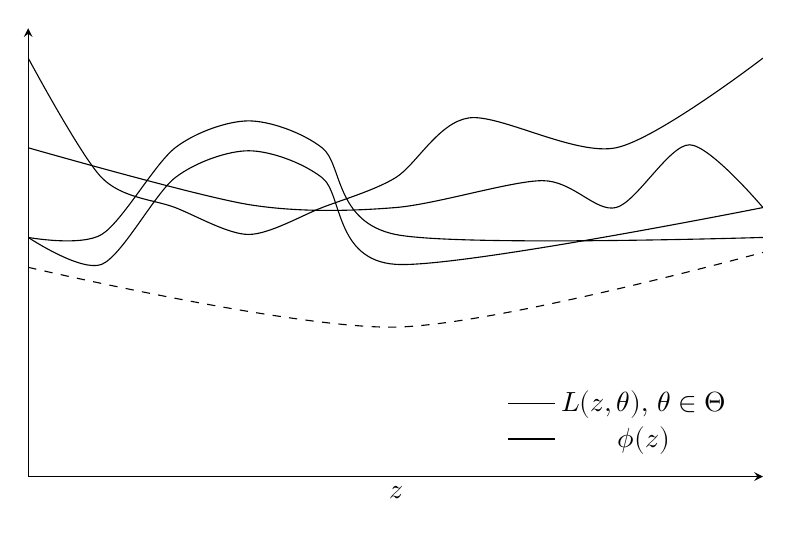
\begin{tikzpicture}
    \begin{axis}[
        ticks=none,
        axis x line=bottom,
        axis y line=left,
        ymin=-4,
        ymax=11,
        xlabel={$z$},
        legend pos=south east,
        legend style={draw=none, fill=none},
        width=0.9\textwidth,
        height=0.6\textwidth,
      ]
      \addplot+[smooth, mark=none, black] coordinates {
        (0, 10) (1, 6) (2, 5) (3, 4.1) (4, 5) (5, 6) (6, 8) (8, 7) (10, 10)
      };
      \addplot+[smooth, mark=none, black] coordinates {
        (0, 4) (1, 4.1) (2, 7) (3, 7.9) (4, 7) (5, 4.1) (10, 4)
      };
      \addplot+[smooth, mark=none, black] coordinates {
        (0, 4) (1, 3.1) (2, 6) (3, 6.9) (4, 6) (5, 3.1) (10, 5)
      };
      \addplot+[smooth, mark=none, black] coordinates {
        (0, 7) (3, 5.1) (5, 5) (7, 5.9) (8, 5) (9, 7.1) (10, 5)
      };
      \addlegendentry{$L(z, \theta)$, $\theta \in \Theta$}
      \addplot+[smooth, mark=none, black, dashed] coordinates {
        (0, 3) (5, 1) (10, 3.5)
      };
      \addlegendentry{$\phi(z)$}
    \end{axis}
  \end{tikzpicture}
\end{figurebox}

\subsection{Nontrivial consistency}


\section{Rate of convergence of learning processes}

\section{Generalization ability of learning processes}

\section{Construction of learning machines}

\subsection{Data classification methods}

\subsection{Regression estimation methods}

\chapter{Machine learning tasks}

In the previous chapter, we define two fundamental inductive learning tasks:
\emph{classification} and \emph{regression}.  In real-world applications, however, we may
require different tasks to solve our data science problem.  Descriptive learning tasks are
out of the scope of this book, I suggest reading \dots. Even restricting ourselves to
discuss only inductive learning, some machine learning tasks comprise a combination of
fundamental tasks.

Also, we show examples of different inductive biases and how the main learning algorithms
work -- symbolic (decision trees), spatial (nearest neighbors), statistical (naïve Bayes
and Bayesian networks), gradient optimization (neural networks.)

\section{Multiclass}

\section{Manifold learning}

\section{Recommender systems}

\section{Reinforcement learning}


\printbibliography

\end{document}
